\documentclass[conference, onecolumn]{IEEEtran} % Replace onecolumn with twocolumn if needed

% Report template for Mälardalen University
% Original template can be found: 
% https://www.overleaf.com/latex/templates/ieee-bare-demo-template-for-conferences/ypypvwjmvtdf
% Template file structure organised by: Emil Persson
% The following packages should follow the IEEE conference guidelines.

% Swedish language package 
\usepackage[utf8]{inputenc}
\usepackage[T1]{fontenc}
\usepackage[swedish,english]{babel}

% Graphics
\usepackage{graphicx, float, subfigure, blindtext}

\newcommand\IEEEhyperrefsetup{
bookmarks=true,bookmarksnumbered=true,%
colorlinks=true,linkcolor={black},citecolor={black},urlcolor={black}%
}

% Preferred hyperref setup, Michael Shell
\usepackage[\IEEEhyperrefsetup, pdftex]{hyperref}

% Maths
\usepackage{mathtools}

% These packages must be at the end
\usepackage[nolist,nohyperlinks]{acronym}
\usepackage{cleveref}
\graphicspath{{images/}}
% \acrodef{acronym}[short name]{full name}
\acrodef{IC}[IC]{Integrated Circuit}
% \acrodef{svm}[SVM]{Support Vector Machine}
\newacro{svm}[SVM]{Support Vector Machine}
% Example use \ac{IC} for printing "Integrated Circuit (IC), use \ac{IC} again and it will print (IC)"
% For plural use \acp{IC} for short and \aclp{IC} for long.
% For more see: http://ftp.acc.umu.se/mirror/CTAN/macros/latex/contrib/acronym/acronym.pdf

% Swedish language package 
\usepackage[utf8]{inputenc}
\usepackage[T1]{fontenc}
\usepackage[swedish,english]{babel}

% Graphics
\usepackage{graphicx, float, subfigure, blindtext}

% \newcommand\IEEEhyperrefsetup{
% bookmarks=true,bookmarksnumbered=true,%
% colorlinks=true,linkcolor={black},citecolor={black},urlcolor={black}%
% }

% Preferred hyperref setup, Michael Shell
% \usepackage[\IEEEhyperrefsetup, pdftex]{hyperref}

% Maths
\usepackage{mathtools}

% These packages must be at the end
\usepackage[nolist,nohyperlinks]{acronym}
\usepackage{cleveref}
\graphicspath{{images/}}

% Remove section first paragraph indent
\usepackage{titlesec}
\titlespacing*{\section}{0pt}{*1}{*1}
\titlespacing*{\subsection}{0pt}{*1}{*1}
\renewcommand{\thesubsubsection}{\arabic{subsubsection}}
\titleformat{\subsubsection}[runin]{\itshape}{\thesubsubsection)}{1em}{}[:]
\titlespacing*{\subsubsection}{\parindent}{0pt}{*1}

% Include authors
\author{\IEEEauthorblockN{
Carl-Johan Höglind\IEEEauthorrefmark{1},
Author 2\IEEEauthorrefmark{2}
}

\IEEEauthorblockA{
School of Innovation, Design and Engineering\\
Mälardalen University, Västerås, Sweden\\
Email:
\IEEEauthorrefmark{1}chd16002@student.mdu.se,
\IEEEauthorrefmark{2}author2@student.mdu.se
}}

% The report title.
\title{Report Title Here\\
Mälardalen University}

% Document begins here
\begin{document}

    % Create the title.
    \maketitle
    % Example sections, name them
    % according to specific needs.
    \section{Question 1} 

    \section{Question 2}
        \subsection{a}
            Sufficient schedulability test for RM scheduling: $U <= n(2^{1/n} - 1)$ \\ where n is the number of tasks in the task set and U is the processor utilization factor, $U = \sum_{i=1}^{n} \frac{C_i}{T_i}$. 

        \renewcommand{\arraystretch}{1.4}
        \begin{figure}[H]
        \centering
        \begin{minipage}{0.5\textwidth}
            \begin{table}[H]
            \centering
            \begin{tabular}{|l|l|l|}
                \hline
                \textbf{Task}   & \textbf{T=D}  & \textbf{C}  \\ \hline
                A               & 3             & 1           \\ \hline
                B               & 5             & 2           \\ \hline
                C               & 2             & 0.5         \\ \hline

            \end{tabular}
            \end{table}
        \end{minipage}%
        \caption{Task set}
        \label{fig:Taskset}
        \end{figure}
    \renewcommand{\arraystretch}{1.0}

        \subsubsection{Task set schedulable?}
        $U = \sum_{i=1}^{n} \frac{C_i}{T_i} = \frac{1}{3} + \frac{2}{5} + \frac{0.5}{2} = 0.98$ \\
        $U <= n(2^{1/n} - 1) = 3(2^{1/3} - 1) = 0.78$ \\
        Since the statement $U <= n(2^{1/n} - 1)$ is false in this case, the task set cannot be proven to be schedulable with this sufficient test method.

        \subsection{b}
            \subsubsection{Exact schedulability test, Tracing}
            \begin{figure}[H]
                \centering
                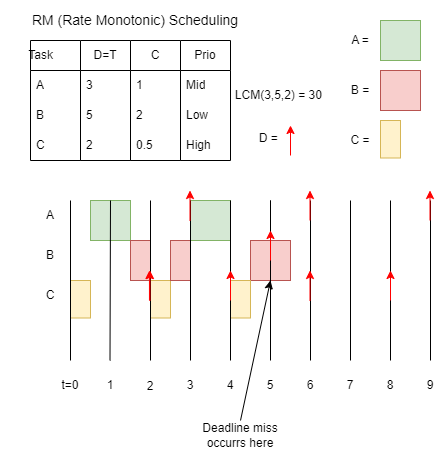
\includegraphics[width=0.5\textwidth]{images/Ass1Q2.drawio.png}
                \caption{Tracing of the task set proves that it is not schedulable with RM.}
                \label{fig:tracing}
            \end{figure}

            As demonstrated in figure \ref{fig:Taskset}, the task set is not schedulable with RM scheduling. The task set is not schedulable because task B misses its deadline at $t = 5$.

    \section{Question 3}

    To calculate the maximum execution time for Task A to make the task set schedulable, the first thing to try is to make the statement $U <= n(2^{\frac{1}{n}} - 1)$ true. In this case $n = 3$ which gives us $U <= 0.78$. So continuing from there we can find the maximum $Ca$ using the equation $U = \sum_{i=1}^{n} \frac{C_i}{T_i}$. The following table contains the given values for period and execution time for the tasks.
    \renewcommand{\arraystretch}{1.4}
        \begin{figure}[H]
        \centering
        \begin{minipage}{0.5\textwidth}
            \begin{table}[H]
            \centering
            \begin{tabular}{|l|l|l|}
                \hline
                \textbf{Task}   & \textbf{T=D}  & \textbf{C}  \\ \hline
                A               & 4             & Ca          \\ \hline
                B               & 12            & 4           \\ \hline
                C               & 20            & 9           \\ \hline
            \end{tabular}
            \end{table}
        \end{minipage}%
        \caption{Task set}
        \label{fig:Q3tasks}
        \end{figure}
    \renewcommand{\arraystretch}{1.0}

    Using the values in the table and the formula $U = \sum_{i=1}^{n} \frac{C_i}{T_i}$ we can extract $Ca$ and get the following equation: $Ca = 4*(0.78 - \frac{4}{12} - \frac{9}{20}) = -0.014ms$. This is not a valid value for $Ca$, so we need to try another approach.\\
    
    We will now try a different approach by finding the worst case execution time (WCET) for task C which is the lowest priority task according to RM scheduling protocols. WCET for task C cannot be slower than $20ms$ because then it will miss its deadline. WCET is found by releasing all higher priority tasks at the same time as task C, but since we do not know the execution time of task A we will only release task B and C and then find the remaining execution time within the $20ms$ period. Within the $20ms$ time period task B will be released twice and execute a total of $2*4ms = 8ms$, task C will be released once and execute a total of $9ms$. If we add up the execution time of task B and C we get $8ms + 9ms = 17ms$. This means that the remaining execution time for task A is a total of $20ms - 17ms = 3ms$. To find the maximum execution time for task A we will have to divide the remaining free time in the $20ms$ period with the number of times task A is released. Task A is released every $4ms$ which means that it will be released $5$ times within the $20ms$ period. The maximum execution time for task A is then $\frac{3ms}{5} = 0.6ms$. So the maximum execution time for task A is $0.6ms$ to make the task set schedulable.

    % We will now try to find maximum $Ca$ by calculating the total amount of execution time needed for all tasks in one hyperperiod. The hyperperiod, or the lowest common multiple (LCM) of the periods of the tasks, is $60ms$. We need to find how many instances occur of each task and then multiply it by the execution time of each task.\\
    % Instances of each task in one hyperperiod:
    % \begin{itemize}
    %     \item Instances of task A: $\frac{LCM}{Ta} = \frac{60}{4} = 15$
    %     \item Instances of task B: $\frac{LCM}{Tb} = \frac{60}{12} = 5$
    %     \item Instances of task C: $\frac{LCM}{Tc} = \frac{60}{20} = 3$
    % \end{itemize}
    
    % The total amount of execution time needed for all tasks in one hyperperiod is then:
    % \begin{itemize}
    %     \item Task A: $15*Ca =?$
    %     \item Task B: $4*5 = 20ms$
    %     \item Task C: $9*3 = 27ms$
    % \end{itemize}

    % We now have the following equation: $15*Ca + 20 + 27 <= 60$. Solving for $Ca$ gives us $Ca <= \frac{60-27-20}{15} = 0.87ms$. This gives us a maximum execution time for task A of $0.87ms$ to make the task set schedulable.\\

    \section{Question 4}
\label{sec:question4}
    
    \section{Question 5}

    To make a task set that is schedulable by EDF but not RM i will find a task set that gives a utilization factor $U = 1$. This will be schedulable with EDF but it is not guaranteed that it is schedulable with RM. To make a task set with $U = 1$ i will use the following equation: $U = \sum_{i=1}^{n} \frac{C_i}{T_i} = 1$. I will use the following task set: 

    \renewcommand{\arraystretch}{1.4}
        \begin{figure}[H]
        \centering
        \begin{minipage}{0.7\textwidth}
            \begin{table}[H]
            \centering
            \begin{tabular}{|l|l|l|}
                \hline
                \textbf{Task}   & \textbf{T=D}  & \textbf{C}  \\ \hline
                A               & 3             & 1           \\ \hline
                B               & 6             & 2           \\ \hline
                C               & 9             & 3           \\ \hline
            \end{tabular}
            \end{table}
        \end{minipage}%
        \caption{Task set}
        \label{fig:Q5tasks}
        \end{figure}
    \renewcommand{\arraystretch}{1.0}

    The task set in figure \ref{fig:Q5tasks} has a utilization factor of $U = \sum_{i=1}^{n} \frac{C_i}{T_i} = \frac{1}{3} + \frac{2}{6} + \frac{3}{9} = 1$. This task set is schedulable with EDF but most likely not with RM. To prove this I will draw the trace for each scheduling algorithm.\\

    \begin{figure}[H]
        \centering
        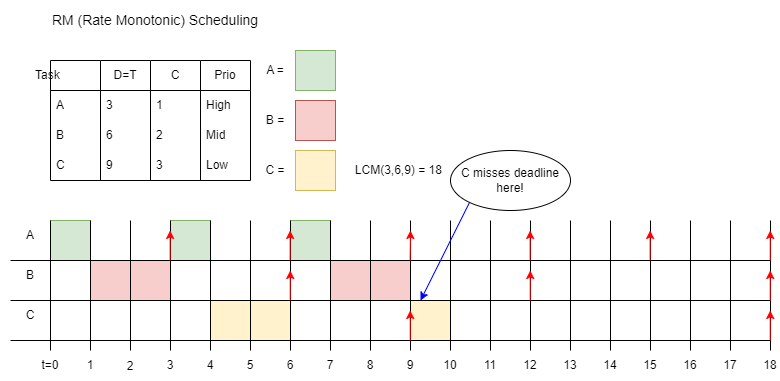
\includegraphics[width=0.8\textwidth]{images/Ass1Q5RM.png}
        \caption{Tracing of the task set with RM scheduling does not work as seen in the figure. The red arrows in the figure indicate the deadlines/period for the tasks.}
        \label{fig:Q5RMtrace}
    \end{figure}

    As seen in figure \ref{fig:Q5RMtrace} the task set is not schedulable with RM scheduling. Task C misses its deadline at $t = 9$.\\

    \begin{figure}[H]
        \centering
        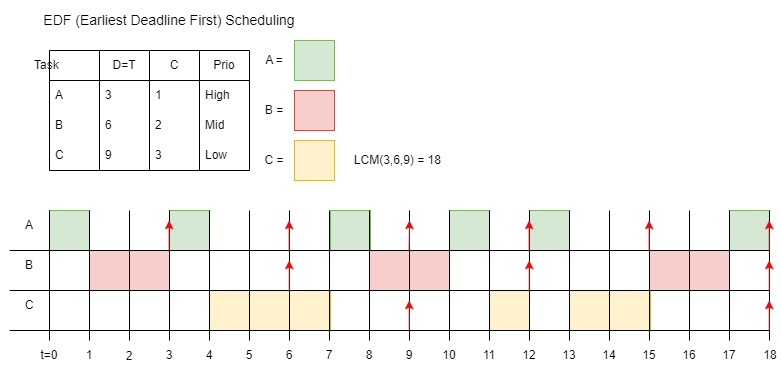
\includegraphics[width=0.8\textwidth]{images/Ass1Q5EDF.drawio.png}
        \caption{Tracing of the task set with EDF scheduling is feasable as seen in the figure. The red arrows in the figure indicate the deadlines/period for the tasks.}
        \label{fig:Q5EDFtrace}
    \end{figure}
        
    As seen in figure \ref{fig:Q5EDFtrace} the task set is schedulable with EDF scheduling. The task set is schedulable with EDF because the task with the earliest deadline is always executed first which guarantees schedulability as long as $U <= 1$.\\
    \section{Question 6}
    \section{Question 7}
    \section{Question 8}


\end{document}